\section{Results}\label{sec-results}
The ethnographic research yielded three main results: (1) an \textit{experimental process workflow}, (2) an \textit{experimental research concept model}, and to a lesser extent, (3) an \textit{experimental process model}. They are described below. We have not used standard notations, e.g., UML or BPMN because experimental researchers (and probably readers) have different ages, backgrounds, and careers. We have valued communication above model formality.

\subsection{Experimental process workflow}

The so-called \textit{experimental process workflow} (EPW) represents the tasks carried out during SE experimentation (according to the RGUS' perspective) and their logical sequence. The workflow is available in this \href{https://zenodo.org/record/7102486#.YyuKruzMLUI}{\ul{link}} and, with lower resolution, it is shown in Fig.~\ref{fig-EPM-construction}.

The EPW model shows three well-defined paths corresponding to the key SE experimental research processes: (1) Experimentation (purple), (2) replication (green), and (3) synthesis (yellow). In addition, based on the existence (or not) of new moderator variables and new knowledge generated in the last round, there are activities of analysis associated with planning new cycles of experimentation, replication, or synthesis and reporting related to the publication of results, respectively (highlighted in blue). Such us processes appear associated with the experimentation and synthesis paths.

\subsubsection{Experimentation path}
Experimentation is the heart of experimental research since replication and synthesis stem from it. However, in some circumstances, experimentation may require the previous execution of synthesis (e.g., when choosing the topic of the experiment) or replication (e.g., in adaptation to the context) activities. According to the experimenters, the experimentation activities are:
\begin{itemize}
	\item Selecting the experiment domain.
	\item Selecting the experiment topic.
	\item Selecting the experimental hypothesis.
	\item Planning the experiment.
	\item Creating the experimental kit.
	\item Executing and post-execution of the experiment.
\end{itemize}

When the experiment results do not meet the experimenters' expectations, they plan a new cycle of experimental research redesigning and conducting the experiment again. This redesign activity usually happens when investigating fundamental topics.

\subsubsection{Replication path}
Replication is the practice on which scientific knowledge is based, hand in hand with the synthesis of results \cite{Roizer-2014-reproducibility}. The RGUS agrees that replication is essential for experimental research both explicitly (RUGS' experimenters claim that) and, more importantly, implicitly (the experimental workflow contains minute details about replication activities). The replication path consists of the following activities: 
\begin{itemize}
	\item Definition of replication.
	\item Study and update the experimental kit.
	\item Adaptation to the context, and
	\item Creation of operational elements.
\end{itemize}

\subsubsection{Synthesis path} 
According to the RGUS experimenters, the synthesis of results can start from systematic literature reviews, systematic mapping studies, or experiments sharing a common goal (a family of experiments). In each case, the experimenters apply particular synthesis techniques (e.g., aggregated or individual patient meta-analysis), followed by interpreting the results. During the interpretation, the researchers can identify moderator variables or generalize pieces of knowledge. Such findings may lead to a reformulation of the synthesis' goal or the conduction of a new cycle of experimental research. In addition, the experimenters generally publish results after a synthesis, hand in hand with planning the next round.

The information obtained from the RGUS looks quite general and in line with the community's understanding of synthesis. That is correct. Our findings are somewhat predictable because the RGUS did not have any experimenter with the required expert knowledge available during this research. On the other hand, the limited insight into synthesis probably represents an indirect confirmation of the ethnographic research's success. Our understanding goes in proportion to the expert knowledge available, and there is a lot of specialized knowledge on the RGUS about experimentation and replication, which was our primary goal. 

\subsection{Experimental research concept model}
This research's conceptual model is not monolithic; on the contrary, it is composed of three sub-models (more accurately, viewpoints) aligned with the prominent experimental roles (research manager - RM, experiment manager - EM, and senior experimenter - SrEx). The activities described in the EPW lead to such views. The experimenters took into account the best-known generic phases of the experimentation process to develop the new versions of the conceptual model (starting from version eight, generated in the first phase of interviews; see \href{https://zenodo.org/record/7102387#.Yyt7W-zMLUI}{\ul{link}}).

\subsubsection{Research manager (RM) viewpoint}
The RM viewpoint is available in this \href{https://zenodo.org/record/7102431#.Yyxi1ezMLUJ}{\ul{link}}. The RM has the following perspective:
\begin{itemize}
	\item In the experiment definition phase, the RM manages the "problem definition" and the "hypothesis definition." 
	\item During the experiment design phase, the RM takes care of the "human resource management" that could "run," "replicate," or be interested in "replicating" the experiment. In addition, the RM receives information regarding the "Expected results," "Execution context," and the "new variables of interest."
	\item While the experiment runs, the RM monitors events. However, the data acquisition phase is transparent to her.
	\item During the data analysis phase, the RM learns the "analysis results" and contributes to the definition of the "findings," "publications," and "pieces of knowledge."
\end{itemize}

\subsubsection{Experiment manager (EM) viewpoint}
The EM viewpoint is available in this \href{https://zenodo.org/record/7102450#.YyxjmezMLUJ}{\ul{link}}. The perspective is as follows:

\begin{itemize}
	\item In the experiment definition phase, the EM actively interacts with all experiment entities, hand in hand with the Senior Experimenter (SrEx). However, in the "hypothesis definition," the EM is only an observer.
	\item In the experiment design phase, the EM focuses on improving the "experiment guides" regarding "instruments," "objects," and the "experimental kit." Additionally, the EM can analyze the context in which the experiment occurs.
	\item During the experiment execution and data acquisition phases, the EM does not lose sight of the "events" that arise and could affect the results. The EM also analyzes the "correctness" of the "collected items" and the "raw data."
	\item In the data analysis phase, the EM cooperates with the "re-analysis" in search of new "variables of interest" to the RGUS. Additionally, the EM can observe the analysis results to suggest findings that could be useful in the publications.
\end{itemize}

\subsubsection{Senior experimenter (SrEx) viewpoint}
The SrEx viewpoint is available in this \href{https://zenodo.org/record/7102464#.Yyxl4ezMLUJ}{\ul{link}}. The perspective is as follows:

\begin{itemize}
	\item In the experiment definition phase, the SrEx observes the "experiment definition," hypotheses' "levels," and "metrics" in the first phase of the experimental investigation. The SrEx participates in the definition of the "hypothesis," "factors," and the "response variable."
	\item In the experimental design phase, the SrEx interacts with a large number of entities; hence, it was necessary to divide such a phase into three sub-phases for this role: \textit{experimental operation design}, \textit{experiment design}, and \textit{artifacts generation}.
    \begin{itemize}
	    \item During the \textit{experimental operation design}, the SrEx defines the "experimental objects" for each "experimental task," considering the minute details of each experimental object's characteristics.
	    \item During the \textit{experiment design} proper, the SrEx establishes the execution context's "parameters," the "design type" with its "groups" and assigned "experimental subjects," the "levels" defined and their combination per "session" and "period," "experimental instruments," and the "measurement procedure." 
        \item Finally, in the \textit{artifact generation}, the SrEx fundamentally develops the "run-kit," which includes the construction of the instances of the "guides," "experimental instruments," and "experimental objects." Such "instances" are the tools that the "subjects" need to participate in the "experiment."
	\end{itemize}
	\item While the experiment runs, the SrEx records all the events produced to analyze their impact on the experiment results.
	\item During data acquisition, the SrEx records the resulting collected items, creates the raw data and obtains measurements.
	\item Finally, in the data analysis phase, the SrEx performs the analysis, obtains the findings, and prepares the publications with the RM and EM's help.
\end{itemize}

\subsection{Experimental process model}
The workflow and the conceptual models represent the experimental research process carried out in the RGUS. Other experimental research groups may work differently. We have created an initial (generic, i.e., generally applicable) experimental process model (EPM) with the help of the most experienced experimenter at RGUS. The model is inspired by the software life cycle \cite{ISO-IEC-IEEE-12207}. We have adapted the concepts used in the ISO/IEC 12207 to the SE experimentation realm. Most of the items have been taken from the EPW (see Figure \ref{fig-EPM-construction}); a lesser portion derives from the conceptual models. The complete process model can be obtained in this \href{https://zenodo.org/record/7105096#.YyxoCOzMLUI}{\ul{link}}.

The EPM contains six groups of processes that define the SE experimental research life cycle: (1) Basic process, (2) Support process, (3) Knowledge item generation process, (4) Publication process, (5) Synthesis process, and (6) Organizational process. 

\subsubsection{Basic process}
The basic process involve fundamental activities that experimenters perform as RM, SrEx, and EM roles before, during, and after running an experiment. Before the experiment, the activities carried out focus on its design, e.g., adapting the experiment to the research context. During the experiment, experimenters pay attention to, e.g., the events that occur before, during, and after the experiment's execution session. The activities performed after the execution focus on the data, e.g., generating raw data and data analysis.

\subsubsection{Support process}
The support process includes activities that the EM performs to manage the materials and support those interested in performing replications, as:

\begin{itemize}
	\item The management of materials before the experiment's execution (e.g., experiment design document), 
	\item the materials used during the experiment (e.g., templates for data collection), 
	\item the materials obtained at the end of the experiment (e.g., filled templates and subjects' code.), and
	\item the Knowledge transference as support style during replication activities.
\end{itemize}

\subsubsection{Knowledge items generation process}
The knowledge items generation process consolidate activities carried out by the RM to manage the knowledge acquired after each experiment, e.g., the knowledge generated in each experimentation phase, the knowledge transferred to professionals, or the knowledge generated during the identification of moderator variables.
   
\subsubsection{Publications process}
This group of activities focuses on reporting the experiment findings (led by the SrEx), aggregation of results (by the EM), and experimentation goals (by the RM).

\subsubsection{Synthesis process}
The EM carries out the synthesis processes. There are different types of synthesis with different evidential levels, e.g., meta-analysis, re-analysis, and informal aggregations.

\subsubsection{Organizational process}
The organizational process include RM's management activities over the SE experimental research cycle, e.g., human resources and publications management. Likewise, the EM also performs management activities on the experiment materials. Finally, there are activities related to synthesis management that have not been assigned to any role yet.

\begin{figure*}[htbp]
\begin{center}
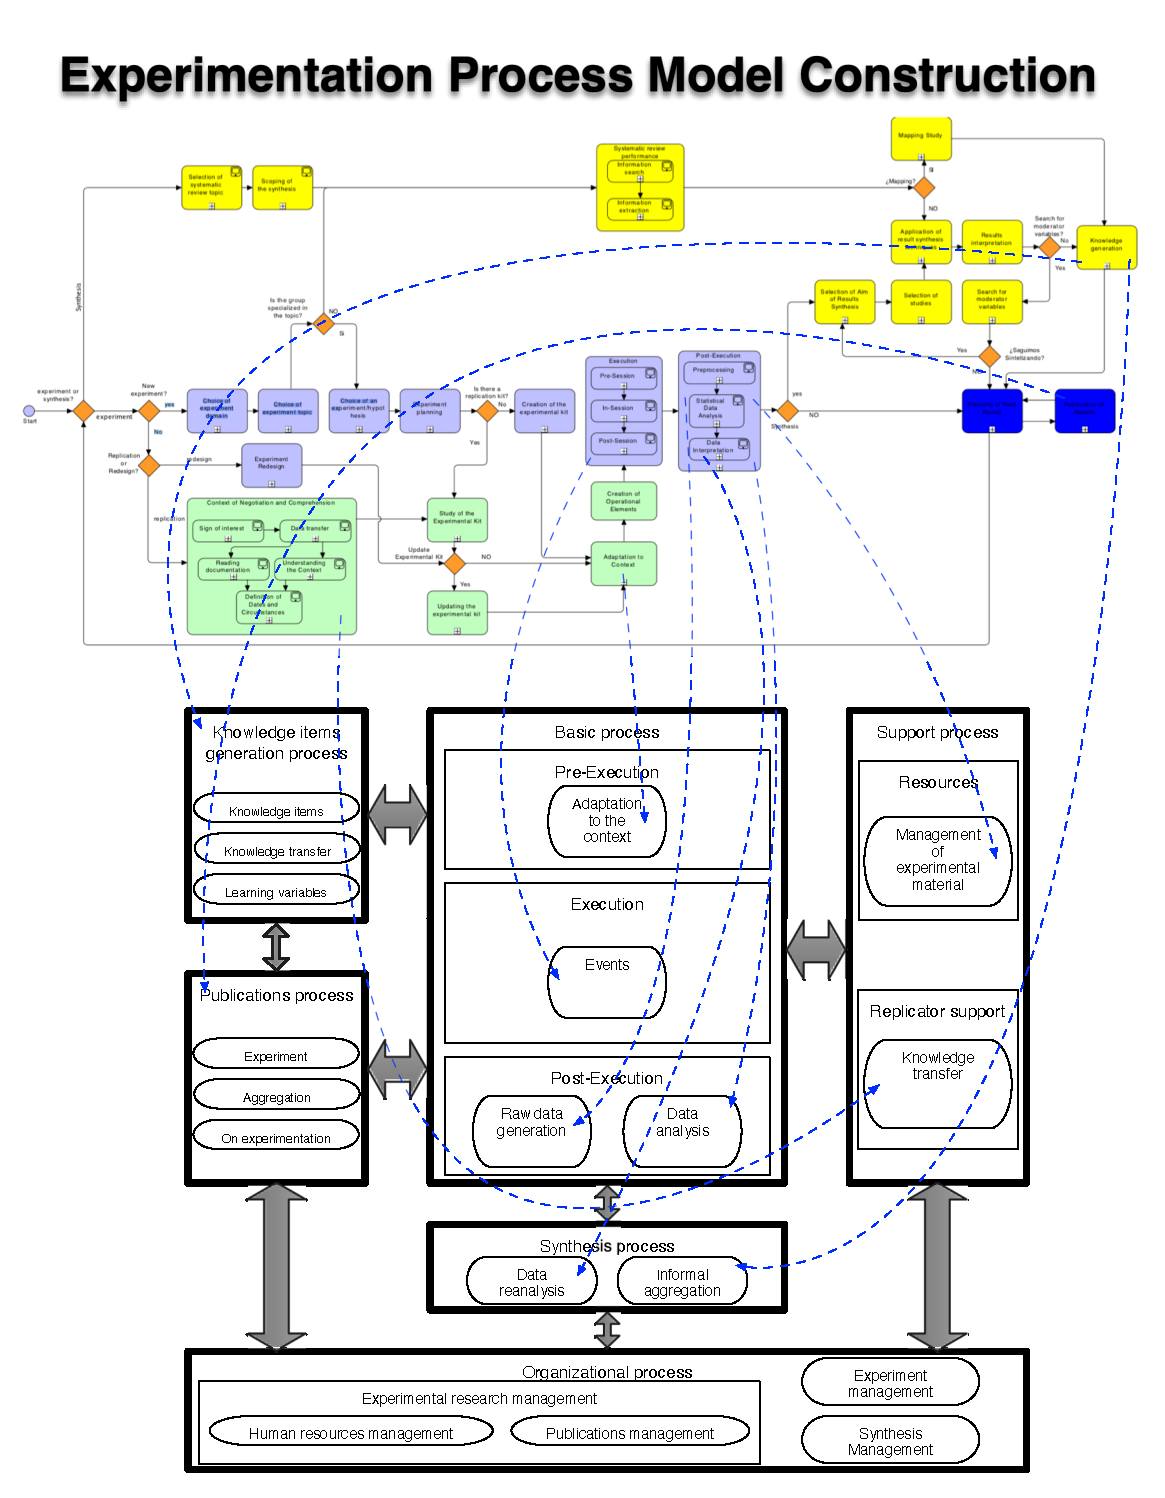
\includegraphics[trim=0 0 0 48,clip,width=0.95\textwidth]{images/Experimentation-Process-Model-Construction}
\caption{Relationships between the \textit{experimental process workflow} (top) and the \textit{experimental process model} (down).}
\label{fig-EPM-construction}
\end{center}
\end{figure*}

Figure \ref{fig-EPM-construction} shows a not very good coincidence between the activities of the EPW and those of the EPM since, as indicated before, each model has its purpose; still, we found several relationships.

Though this model is plausible, it is based on the RGUS' perspective alone. Further research (in this regard, see Section~\ref{sec-conclusions}) is necessary to ensure that the model represents the experimental SE community's experimental process. 